\scanpage{73}\mspage{72}

sous-figure de \deleted{$\unsure{G'|F'}$} la subdivision $F'$ de $F$, induite par la sous-figure $\deleted{F}G$ de $F$.
% slanted: three oblique lines, the third beginning with the low, detached de.
\margin{\unsure{double} \unsure{Transitivité} de l'induction}

$\uline{C}7_0$ Pour toute figure $F$, sous-figure $G$, et subdivision $G'$ de $G$, il existe une subdivision $F'$ de $F$ qui induise $\unsure{C'|G'}$\unsure{,|.}

% ROOT-FIG-PARENTHESIS: the paragraph is grouped to preserve the q-descender
% adjoining the worked mark before the first order, and the crossed curled mark.
% The first graphic admits a cancelled l/F or a retraced end of q; no extra
% complete letter is asserted. The second admits a cancelled parenthesis or a
% worked punctuation sign. Both are preserved as doubt-marked actual strokes.
\figure{\begin{tikzpicture}[every node/.style={inner sep=0pt,anchor=base west},font=\small]
\node (pprefix) at (0,0) {(mais l'énoncé symétri};
\node (pq) at (pprefix.base east) {q};
\node at (pq.base east) {ue, où on};
\node (roles) at (0,-.62) {échangerait les rôle de};
\node (pmark) at ([xshift=.12cm]roles.base east) {\unsure{\begin{tikzpicture}[x=.07cm,y=.07cm,baseline=0pt]
\draw[line width=.5pt] (0,4.5) .. controls (.3,3) and (.1,1) .. (.7,0);
\draw[line width=.5pt] (.1,1.1) -- (2.6,4.8) .. controls (2.8,3.5) and (1.3,2.4) .. (.5,1.2);
\draw[line width=.5pt] (.5,1) -- (1.7,1);
\end{tikzpicture}}};
\draw[line width=.35pt] ([xshift=.02cm]pq.south) .. controls ([xshift=.07cm,yshift=-.15cm]pq.south) and ([xshift=.1cm,yshift=.15cm]pmark.north west) .. ([xshift=.04cm]pmark.north west);
\node at ([xshift=.08cm]pmark.base east) {$\leq$ et $\preceq$,};
\node (faux) at (0,-1.25) {est faux};
\node (curl) at ([xshift=.13cm]faux.base east) {\unsure{
\begin{tikzpicture}[x=.025cm,y=.025cm,baseline=-.1ex,line width=.5pt,line cap=round,line join=round]
\draw (3,19) .. controls (4,23) and (6,22) .. (7,19);
\draw (3,20) .. controls (2,16) and (2,13) .. (4,11)
 .. controls (3,8) and (7,8) .. (8,8)
 .. controls (10,7) and (5,3) .. (4,0);
\draw (2,20) -- (5,9);
\draw (1,16) .. controls (0,12) and (2,11) .. (6,12);
\draw (0,15) -- (7,12);
\draw (4,12) .. controls (6,17) and (10,21) .. (13,22);
\end{tikzpicture}}};
\node at ([xshift=.08cm]curl.base east) {: il n'est pas vrai, pour};
\node at (0,-1.92) {$F'\preceq F$ donnés, que tte sous figure $G'$ de};
\node at (0,-2.56) {$F'$ \unsure{soit|sont} induite par une ss-figure $G$ de $\deleted{G}F$).};
\end{tikzpicture}}

On \deleted{peut} renforcera par la suite $C7_0$ en
% ROOT-MARK-BEFORE-C7: one short curved stroke, with no secure independent strike.
\unsure{\begin{tikzpicture}[x=.045cm,y=.045cm,baseline=0pt]
\draw[line width=.5pt] (1.6,3.2) .. controls (1.8,1.8) and (1.1,.8) .. (0,0);
\end{tikzpicture}}$C7$, en prenant un choix canonique de $F'$.

% ROOT-FIG-DRAFT. All text is written once.
% The last resulte is unaccented; its line-level doubt concerns
% only cancellation scope, not the letters or the double arrow. The three broad oblique cancellation
% strokes, local title cancellation, insertion enclosure, and local C6-line
% cancellation are drawn at their actual relative positions. The final C7_0
% line is below every diagonal endpoint; its uncertainty concerns the extent
% of the block cancellation, not its words or its double arrow.
\figure{\begin{tikzpicture}[x=.009cm,y=-.009cm,every node/.style={inner sep=0pt,anchor=base west},font=\small]
\node at (310,1555) {\unsure{Corollaire|Comparabilité} \unsure{1}};
\draw[line width=.6pt] (315,1611) -- (630,1602);
% The separate dense title cancellation, distinct from the three long strokes.
\draw[line width=.55pt] (354,1582) -- (372,1510) -- (363,1585) -- (397,1520) -- (376,1588) -- (416,1528) .. controls (398,1593) and (410,1592) .. (440,1535) .. controls (429,1604) and (443,1601) .. (481,1519) .. controls (455,1611) and (475,1600) .. (529,1532) .. controls (510,1613) and (518,1610) .. (606,1520) .. controls (584,1596) and (601,1581) .. (680,1517) .. controls (667,1567) and (688,1542) .. (711,1555) -- (709,1581);
\node at (840,1548) {Soient $F,\deleted{A}G$ deux figures.};
\node at (300,1637) {\inserted{Considérons les}};
% ROOT-INSERTION-ENCLOSURE: the full raised phrase, not only Considérons.
\draw[line width=.45pt] (310,1704) .. controls (298,1673) and (329,1651) .. (365,1653) .. controls (475,1642) and (623,1641) .. (686,1624) .. controls (697,1620) and (690,1608) .. (686,1600);
\node at (328,1685) {Conditions \deleted{équivalentes} :};
\node at (407,1750) {a) $G$ est une sous-figure d'une subd. de $F$ :};
\node at (722,1856) {\begin{minipage}{3cm}\[G\leq F'\preceq F\]\end{minipage}};
\node at (400,1934) {b) $G$ est une subdivision d'une sous-};
\node at (350,2010) {figure de $F$ :};
\node at (691,2088) {\begin{minipage}{3cm}\[G\preceq G'\leq F.\]\end{minipage}};
\node at (372,2144) {On a alors b) $\Rightarrow$ a)};
\node at (985,2118) {(Mais pas \unsure{vrai|vice}\unsure{,} a $\Rightarrow$ b !!!};
% ROOT-CLOSING-TICK: a closing parenthesis with a tiny attached side stroke;
% no separate baseline full stop is supplied.
\draw[line width=.5pt] (1601,2053) .. controls (1636,2071) and (1640,2113) .. (1604,2131);
\draw[line width=.35pt] (1629,2089) -- (1634,2088);
\node at (367,2218) {a) $\Rightarrow$ b) résulte de C6};
\draw[line width=.65pt] (370,2224) -- (1079,2189);
\node at (371,2285) {\unsure{b) $\Longrightarrow$ a) resulte de $C7_0$}};
% ROOT-DIAG-SQUARE. The relation, cup, bottom points and right endpoint retain
% their graphic forms; the large diagonal belongs to the block cancellation.
\node[anchor=north west] at (1290,2120) {\begin{minipage}{2.5cm}
\diagram{\begin{tikzcd}[ampersand replacement=\&,column sep=2.0em,row sep=1.1em]
F \arrow[r,phantom,"{\unsure{\begin{tikzpicture}[x=.025cm,y=.025cm,baseline=0pt]
\draw[line width=.5pt] (0,3.5) -- (4.5,6.8);
\draw[line width=.9pt] (0,2.2) .. controls (5.8,1.8) and (8,6.4) .. (7.1,10.3);
\draw[line width=.65pt] (3.9,3.0) .. controls (7.8,4.4) and (9.1,6.8) .. (9.3,8.7);
\draw[line width=.8pt] (0,2.2) .. controls (5,2.2) and (8,1.9) .. (9.3,0);
\draw[line width=.55pt] (.8,-.3) .. controls (5.5,-.1) and (7.5,-.7) .. (8.5,-1.8);
\end{tikzpicture}}}" description]
\arrow[d,phantom,"{\unsure{\cup|U}}" description]
\& F' \arrow[d,phantom,"{\begin{tikzpicture}[x=.03cm,y=.03cm,baseline=0pt]
\draw[line width=.6pt] (0,6.1) .. controls (.5,5.4) and (.2,5.1) .. (0,4.8);
\fill (-.2,3.5) circle[radius=.25];
\fill (.35,3.0) circle[radius=.23];
\fill (.2,2.5) circle[radius=.23];
\draw[line width=.65pt] (-1,1.7) -- (-.7,.8) -- (.1,0) -- (1.2,.8) -- (1.0,1.8);
\draw[line width=.45pt] (-.7,.8) -- (.8,1.7) -- (-.8,1.3);
\end{tikzpicture}}" description] \\
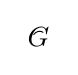
\begin{tikzpicture}[x=1ex,y=1ex,baseline=-.4ex]
\node[inner sep=0pt] at (0,0) {$G$};
\draw[line width=.35pt] (-.42,.20) .. controls (-.22,.52) and (.16,.55) .. (.40,.40);
\end{tikzpicture}
\arrow[r,phantom,"{\cdots}" description] \& G'
\end{tikzcd}}
\end{minipage}};
% The three continuous oblique strokes, including the short far-right stroke.
\draw[line width=.45pt] (444,1538) .. controls (504,1740) and (694,2047) .. (793,2212);
\draw[line width=.5pt] (1034,1479) .. controls (1060,1628) and (1301,2029) .. (1423,2233);
\draw[line width=.3pt] (1399,1491) .. controls (1470,1594) and (1552,1755) .. (1598,1849);
\end{tikzpicture}}
